\chapter{Propuesta}
\label{chap5}
\ifpdf
  \graphicspath{{Chapter5/Chapter5Figs/PNG/}{Chapter5/Chapter5Figs/PDF/}{Chapter5/Chapter5Figs/}}
\else
  \graphicspath{{Chapter5/Chapter5Figs/EPS/}{Chapter5/Chapter5Figs/}}
\fi

\markboth{\hfill \thechapter. Propuesta}{\hfill \thechapter. Propuesta}

\section{Planteamiento del problema}
\label{sec:planteamiento}

Encontramos un factor común en varios artículos leídos y nuestro caso de estudio, donde el conductor es quien, a base de su experiencia, selecciona el camino a seguir para la recolección de residuos urbanos (Akhtar, 2017; Braier, 2017; Düzgün, 2016) \citet{Akhtar2017BacktrackingOptimization, Braier2017AnArgentina, Duzgun2016ParallelRouting}, dejando algunas veces sin servicio algunos puntos de la ciudad. Es por ello que nos centraremos en resolver la ruta óptima del recorrido de los camiones recolectores desde que sale de la DSU, recoge los residuos dentro de su zona asignada, deposita los residuos en el vertedero de Cateura y hasta que regresa nuevamente a la DSU, para evitar duplicaciones en el paso del camión por las mismas cuadras varias veces en el día.

En ocasiones las calles cambian de sentido o son clausuradas por refacción u otros motivos por un cierto periodo de tiempo. Por lo tanto, proponemos la implementación de un prototipo de sistema GIS, en donde se podrán modificar los parámetros de entrada, aplicar el algoritmo y generar las rutas óptimas a partir de ellos.

\begin{figure}[H]
    \centering
    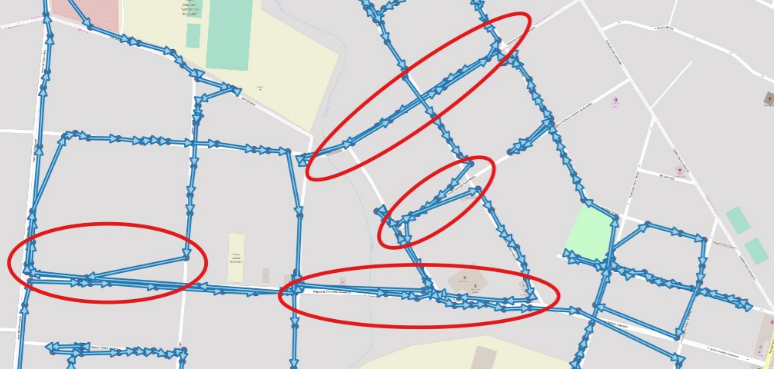
\includegraphics[width=14.5cm]{20170329_recorrido_repetido.png}
    \caption{Trayecto del vehículo 62 en fecha 11 de Julio del 2016 en el turno mañana. [Fuente: Datos de rastreo vía GPS desplegados en la aplicación QGis]}
    \label{fig:trayectoRecoleccion}
\end{figure}

En la Figura \ref{fig:trayectoRecoleccion}, se muestra una pequeña parte del rastreo de una zona, en los círculos de color rojo se pueden observar como el mismo vehículo recorre la misma calle más de una vez. Esta situación se pudo contemplar en los recorridos de varias zonas. Para la recolección de datos se solicitó a la DSU el permiso de instalar un dispositivo GPS a un vehículo recolector de basura, como parte de este proyecto, a través del cual obtuvimos por un periodo de 3 meses los datos de posicionamiento relacionados al vehículo 62 de propiedad de la Municipalidad de Asunción. Esta idea ya generó el interés de la Municipalidad de Asunción, que posteriormente ha realizado una licitación para dotar a todos los vehículos recolectores de residuos un dispositivo similar GPS, brindándonos acceso a los datos del rastreo de todos vehículos recolectores.

\subsection{Solución planteada}

La solución del trabajo de investigación es lo que se buscará encontrar en el transcurso del desarrollo del TFG. La solución encontrada debe permitir obtener mejores resultados en cuanto a costo de recolección, en comparación a la situación actual en la DSU del municipio de Asunción, así como también, generar resultados óptimos que contribuyan con el estado del arte actual












